% file siminos/froehlich/slice/singul.tex
% $Author$ $Date$

% \section{\Sset}
%	\label{sec:singul}

If  two patterns are close, their group orbits are nearly parallel,
$\braket{\groupTan(\ssp)}{\sliceTan{}} \neq 0$, and a slice is transverse
to all group orbits in an open neighborhood of the {\template} \slicep.
However, globally the \mslices\ always introduces singularities. Two
hyperplanes are associated with  any given {\template} \slicep; the slice
\refeq{PCsectQ}, and the hyperplane of points \sspSing\ such that from
the {\template} vantage point their group orbits are not transverse, but
locally `horizontal,'
\beq
\braket{\groupTan(\sspSing)}{\sliceTan{}}
 =
\braket{\sspSing}{\Lg^2\slicep}
 =0
%\,.
\ee{sliceSingl0}
(for simplicity, in this section we specialize to the  $\SOn{2}$ case).
We shall refer to the $(d\!-\!2)$\dmn\ intersection of the two as the
{\em \sset} $S$,
\beq
\braket{\groupTan(\sspRSing)}{\sliceTan{}}
 =
\braket{\sspRSing}{\Lg^2\slicep}
 =0
\,.
\ee{sliceSingl}
Looking back at \refeq{SO2inflPoint}, we see that $S$ is the locus of
inflection points, a hyperplane through which the curvature of the
distance function changes sign, and a local minimum turns into a local
maximum.  For example, for \cLe\ $\sspRSing =
(x_1^*,x_2^*,y_1^*,y_2^*,z^*)$, $\slicep = (x_1',x_2',y_1',y_2',z')$, and
the 3\dmn\ {\sset} $\sspRSing \in S \subset \pSRed$ is given by vanishing
denominator in \refeq{braketCL}:
\[
0 = {x_1^* x'_1+x_2^* x'_2+y_1^* y'_1+y_2^* y'_2}
\,.
\]
The {\sset}  $S$ is purely an artifact of the choice of a {\template},
and has nothing to do with the dynamics; whenever the full \statesp\
trajectory crosses an {\sset}, it pays it no heed whatsoever.

We next show that the singularity in
the formula \refeq{SL:CLEsliceRot} causes a discontinuous jump in the
moving frame angle $\gSpace$. Consider a full \statesp\ trajectory
$\ssp(\tau)$ that passes through the {\sset} \refeq{sliceSingl} at time
$\sspRSing =\ssp(\tau^*)$, which we shall set to  $\tau^*=0$. At that
instant the moving frame angle $\gSpace$ is formally undefined: the
numerator $\braket{\sspRSing}{\sliceTan{}}$ in \refeq{SL:CLEsliceRot}
vanishes ($\sspRSing$ is in the slice and satisfies the slice condition
\refeq{PCsectQ}), and the denominator
${\braket{\groupTan_{}(\sspRSing)}{\sliceTan{}}}$ vanishes by
\refeq{sliceSingl}. Nevertheless, the trajectory going through the singularity
is well defined, as in the linear approximation the numerator and the
denominator in the moving frame formula \refeq{SL:CLEsliceRot} are given
by
\bea
\braket{\ssp}{\sliceTan{}}
    &=&
\braket{(\sspRSing+\vel(\sspRSing) \, \tau ))}
       {\sliceTan{a}}
    \,=\,  \braket{\vel(\sspRSing)}
       {\sliceTan{a}} \, \tau
	\label{singSetVelo}\\
\braket{\groupTan(\ssp)}{\sliceTan{}}
    &=&
\braket{\groupTan(\sspRSing+\vel(\sspRSing) \, \tau ))}
       {\sliceTan{a}}
    \,=\, \braket{\groupTan(\vel(\sspRSing))}
       {\sliceTan{a}} \, \tau
\,.
\label{singSetSign}
\eea
In other words, the moving frame rotates the \statesp\ point $\ssp$ and
the velocity $\vel(\ssp)$ by the same angle, so either can be used to
compute it. The infimum in the slice condition demands that we pick the
solution with positive curvature \refeq{SO2inflPoint}, so
$\braket{\groupTan(\ssp)}{\sliceTan{}}\geq 0$
for all $\tau$. As the trajectory traverses $\sspRSing$, the time $\tau$
changes the sign from negative to positive; hence we must switch from the
solution $\sspRSing$ to another extremum for which
$\braket{\groupTan(\vel(\sspRSing))}{\sliceTan{}}$ is positive. In the
\cLf\ example there are only two extrema $\{\gSpace,\gSpace+\pi\}$,
so the moving frame angle $\gSpace$ jumps discontinuously by $\pi$.

Within the \reducedsp\  an {\sset} crossing has a dramatic effect: the
\reducedsp\ flow $\sspRed(\tau)$ \emph{jumps} whenever it crosses the
{\sset} $\sspRSing$, by amount that we now compute.
Suppose that a \reducedsp\ trajectory passes through a singularity
$\sspRSing$ at time $\tau=\tau^*$. At
that instant the numerator $\braket{\vel(\sspRSing)}{\sliceTan{a}}$ is
(generically) finite, but as the group tangent of the point $\sspRSing$
lies in the slice, ${\braket{\groupTan_{}(\sspRSing)}{\sliceTan{}}}=0$
by \refeq{sliceSingl}, the denominator in \refeq{eq:so2reduced} vanishes,
and the {\angVel} $\dot{\gSpace}$ shoots off to infinity.
\SF{For the nearby trajectories the numerator is nonzero, but along a trajectory passing
through a singularity doesn't the numerator approach zero $\gSpace$ approach the angle required
to rotate the velocity into the slice. Hence the infinitely thin delta function}

% 2010-12-20 previously {CLEsingpass}{CLEnearsing2}
 \begin{figure}
 \begin{center}
(a) 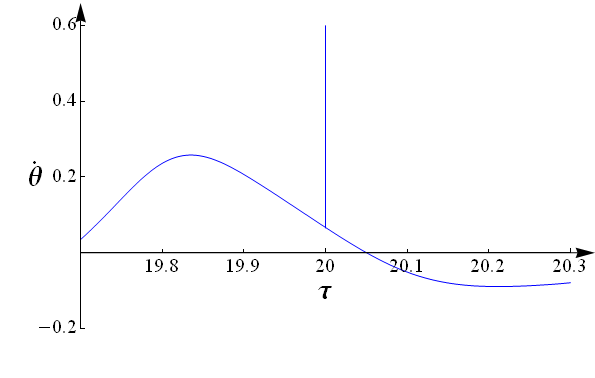
\includegraphics[width=0.35\textwidth]{dthetasing}%
~~
(b) 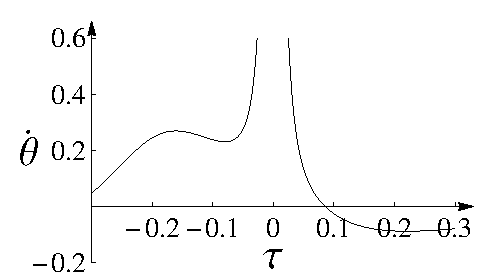
\includegraphics[width=0.35\textwidth]{dthetanearsing}%
 \end{center}
 \caption{\label{fig:dthetasing}
The {\angVel} $\dot{\gSpace}$ for two \cLf\
\reducedsp\ trajectories in a slice defined by the
{\template} $\slicep$ given in \refeq{exmplTempl}:
 (a) As the trajectory $\sspRed(\tau)$ passes through the
singular point  $\sspRSing$ given in \refeq{exmplTempl},
the {\angVel} diverges
$\dot{\gSpace} \to \infty$ as a Dirac delta function.
(b) The {\angVel} for a nearby trajectory going
through $\sspRSing+\delta \ssp$,
$\delta\ssp=(0.01,0,0,0,0)$ exhibits a large
but finite excursion close to the singularity.
 }%
 \end{figure}

As an illustration of such jump, consider a blow-up of the small rectangle indicated
in \reffig{fig:Fullspace}\,(b). Here the {\template}
	\PC{to SF - Please provide this secret numbers!}
\bea
\slicep 	&=& (0.887846,-0.150461,0.4,-0.12,0)
	\continue
\sliceTan{} &=& (0.150461,0.887846,0.12,0.4,0)
	\label{exmplTempl} \\
\sspRSing	&=& (-0.889135, -0.0401956, 1.91332, -0.150327, 24.4436)
\nnu
\eea
was reverse-engineered, by picking a point $\sspRSing = \ssp(0)$ from a
segment of the full \statesp\ ergodic trajectory $\ssp(\tau)$ and then
computing \slicep\ such that $\sspRSing$ lies in the {\sset}. As the
trajectory $\sspRed(\tau)$ passes through the $\sspRSing$, the {\angVel}
diverges $\dot{\gSpace} \to \infty$ as a Dirac delta function,
\reffig{fig:dthetasing}\,(a), and the \reducedsp\ trajectory goes through
the inflection \refeq{sliceSingl} and jumps to the $\pi$-rotated extremum
of the distance function, \reffig{fig:singpass}\,(a).
	\PC{no need to use color in \reffig{fig:dthetasing}, make it B\&W.}

The {\sset} $S$ is the intersection of two hyperplanes: (1) the slice
(infimum of the group-orbit distance to the {\template}), and (2) the
closest inflection in the distance function \refeq{sliceSingl}, and thus
of higher codimension than either. While all group orbits of a  generic
trajectory cross the slice, the trajectory has vanishing probability to
cross the lower-dimensional {\sset} - that is why we had to `engineer'
the slice \refeq{exmplTempl}. However, an ergodic trajectory  might come
arbitrarily close to  $S$ arbitrarily often.
	\PC{This hopefully resolves a long-standing conundrum for Evangelos
        and me. Please CORRECT ME if I am wrong, I'm on thin ice here!}
Such nearby \reducedsp\ trajectories exhibit large {\angVels} $\dot{\gSpace}$,
\reffig{fig:dthetasing}\,(b), and very fast, nearly semi-circular
excursions close to the singularity, \reffig{fig:singpass}\,(a). Which segment
of the group orbit they follow depends on the side from which the
trajectory approached the {\sset}.
	\PC{to Stefan: In \reffig{fig:dthetasing}\,(b) and \reffig{fig:singpass}\,(a)
you use a full \statesp\ perturbation $\delta \ssp$. Would it be more consistent
to perturb with $\delta \sspRed$?}
    \SF{I used the perturbation $\delta \ssp$ because I was calculating the trajectories in the full space and then reducing them. dy=(-0.0246486, 0.00417712, 0., 0., 0.) if you want to use it}

% 2011-01-12 previously Figs. {singpass} and {fig:Tesselate}
% In FrCv11.tex replaced by f_1_08_1.png
%{Hyp} %{fig6} and {tr:fig6} in ChaosBook
% \HREF{http://chaosbook.org/overheads/trace/Tesselate.jpg}
 \begin{figure}
 \begin{center}
(a) 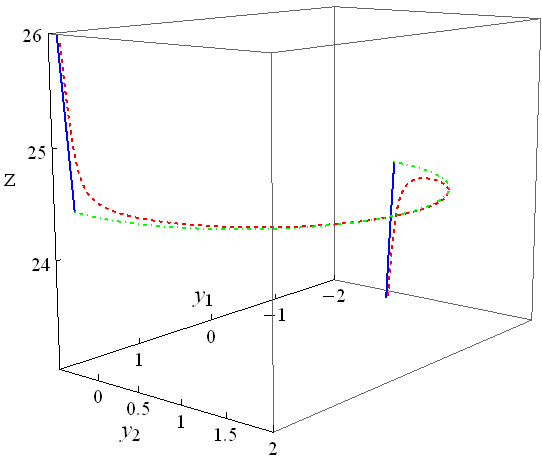
\includegraphics[width=0.32\textwidth]{singpass1}%
~~~~
(b)~ 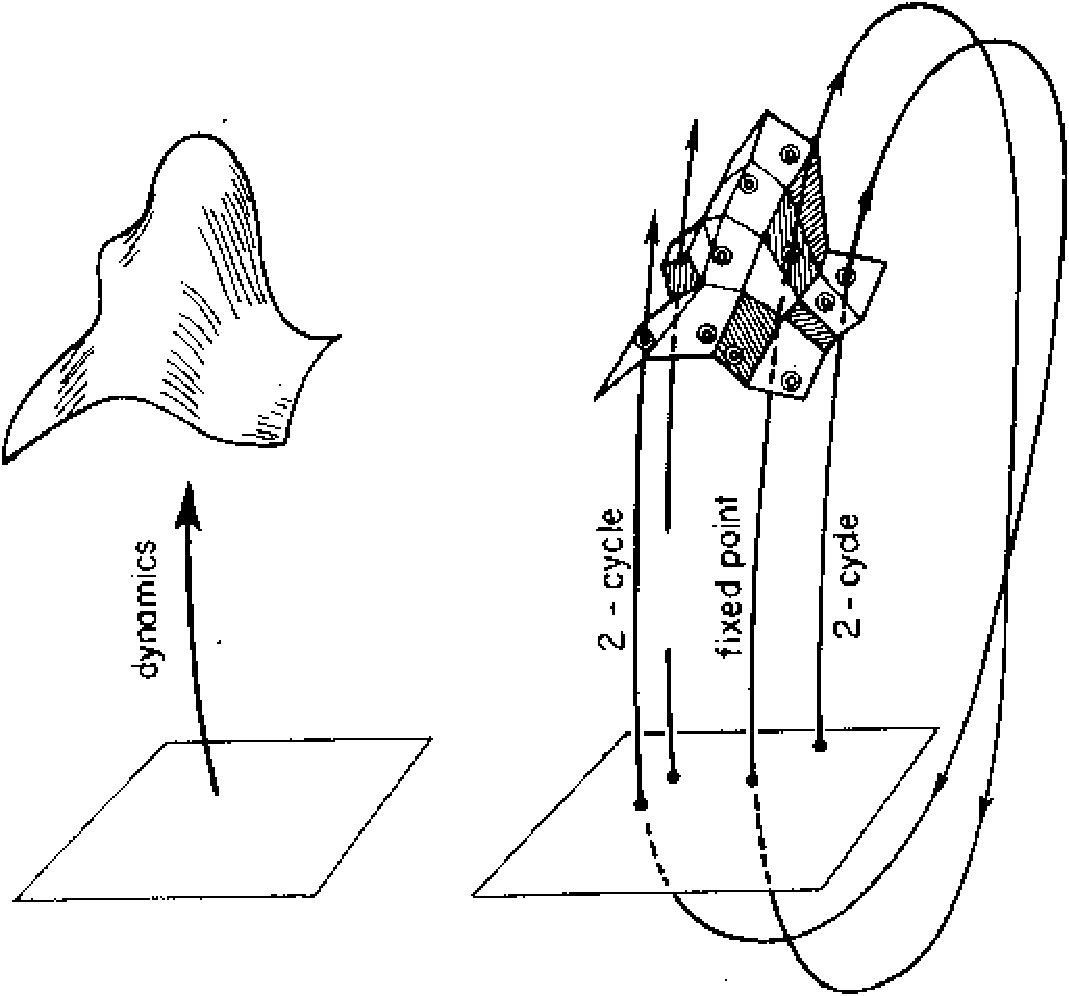
\includegraphics[width=0.40\textwidth]{f_1_08_1}
 \end{center}
 \caption{\label{fig:singpass}
(color online).
(a)
Blow-up of a jump in \reffig{fig:Fullspace}\,(b), indicated by a small
rectangle.
(blue/dotted) A trajectory that passes through the singular point
$\sspRSing$ given in \refeq{exmplTempl}. Note the instantaneous jump in
the trajectory,  caused by the divergence in velocity
(\reffig{fig:dthetasing}\,(a)) as the trajectory traverses the {\sset}.
The neighboring red/dashed trajectory going through $\sspRSing+\delta
\ssp$, $\delta \ssp =(0,0.025,0,0,0)$, makes a rapid transit around the
singularity. The green trajectory is the group orbit of $\sspRSing$
between the two $\gSpace$ that rotate $v(\sspRSing)$ in the slice. Note
also how the red/dashed trajectory begins near the blue/dotted
trajectory, closely follows the green trajectory after the singularity
point, reaches the other side of the blue/dotted arc and then resumes
closely following the blue/dotted trajectory.
(b)
Smooth dynamics  (left frame) tesselated by the skeleton of periodic
points, together with their linearized neighborhoods, (right frame).
Indicated are segments of two 1-cycles and a 2-cycle that alternates
between the neighborhoods of the two 1-cycles, shadowing first one, and
then the other
(from \wwwcb{}).
 }%
 \end{figure}

In summary, whenever a \reducedsp\ trajectory crosses the {\sset}, it
jumps instantaneously and discontinuously to the new distance infinum. We
have shown that these jumps are harmless and theoretically under control.
Nearby trajectories are numerically under control if sufficient care is
taken to deal with large \angVels. But they are an artifact of the
\mslices\ of no dynamical significance, and an uncalled-for numerical
nuisance. We now outline a strategy how to avoid them altogether by a
clever choice of {\template s}.

%
% ****** End of file singul.tex ******
